% mainfile: ../RobertoDiRemigioPhDThesis.tex
%************************************************
\chapter{Summary of the publications}\label{ch:publications-summary}

\epigraph{$\frac{1}{2}$ research and $\frac{1}{2}\,\,T\acute{\epsilon}\chi\nu\eta$

          $\frac{1}{2}$ observation, $\frac{1}{2}\,\,T\acute{\epsilon}\chi\nu\eta$

          $\frac{1}{2}$ training, $\frac{1}{2}\,\,T\acute{\epsilon}\chi\nu\eta$}{
  --- \textsc{Ezra Pound}, \textit{Canto LXXXV}}

In the following, I provide a brief summary of the motivations, contents and
conclusions of the papers this thesis is based on.
Figures and tables here reported are minimally modified versions taken from the published work,
captions are instead copied \emph{verbatim}.
In addition, I give a description of my contributions to the work leading to
the publication of each of the papers.
\todo[inline]{Write something along these lines: "My coauthors have all read and approved."}

\section*{Software}

The codes used in the papers are all interfaced to the \pcmsolver library,
of which I am the main developer and maintainer.

\refstepcounter{dummy}
\addcontentsline{toc}{section}{Continuum solvation in the relativistic regime}
\section*{Paper I. Continuum solvation in the relativistic regime}

Systems containing heavy elements are notoriously challenging for quantum chemistry.
In addition to their significantly large sizes, one has to properly include the
effect of special relativity in the quantum chemical description in order to
achieve at least qualitative agreement with experiment.
Additional complications arise if one needs to also include environment effects.
Continuum models arguably represent a cost-effective strategy to achieve a first
approximation of these effects.
In this paper, we presented the first derivation and implementation of the \acs{PCM}
coupled to a \acs{SCF} description of the solute in the fully relativistic, four-component
regime.
Our preliminary calculations on the group 16 dihydrides \ce{H2X} (\ce{X} =
\ce{O}, \ce{S}, \ce{Se}, \ce{Te}, \ce{Po}) have shown that the method predicts
a noticeable interplay of relativistic and solvent effects when heavier
elements are involved.
The main point of the paper was, however, the adoption of a fully modular
programming strategy. We showed that it is entirely possible to adopt the same
\acs{PCM} code and implementation "checkpoints" across altogether different
problem domains.

\begin{figure}[!htb]
\centering
\scalebox{0.8}{\tikzstyle{decision}=[diamond, fill=red!20, text width=5.5em, text badly centered, inner sep=0pt]
\tikzstyle{pcmsolver}=[rectangle, minimum size=6mm, rounded corners=3mm, very thick, fill=Blue!20, text width=14em, text centered]
\tikzstyle{qmprog}=[rectangle, minimum size=6mm, rounded corners=3mm, text centered, very thick, fill=Green!20, text width=14em]

\begin{tikzpicture}[]
%skip up/.style={to path={-- ++(0,#1) -| (\tikztotarget)}},
%skip right/.style={to path={-- ++(#1,0) -| (\tikztotarget)}}]
\node (MEP) [qmprog] { Molecular electrostatic potential at the cavity: \\ $
 v_I = \sum_A \frac{Z_A}{|\vect{R}_A-\vect{s}_I|} +  \sum_{\kappa\lambda} D_{\lambda\kappa}
\left[\int\diff\vect{r}\frac{-\Omega_{\kappa\lambda}(\vect{r})}{|\vect{r}-\vect{s}_I|}\right]$ };
\node (CHG) [pcmsolver, below=of MEP] { Apparent Surface Charge:\\ $\vect{q} = \mat{K} \vect{v}$ };
\node (energy) [pcmsolver, below=of CHG] { Polarization energy:\\ 
$U_\mathrm{pol} = \vect{q}\cdot\vect{v}$};
\node (fock) [qmprog, below=of energy, distance=30mm] { Fock matrix:\\
$f_{\kappa\lambda} = f^\mathrm{vac}_{\kappa\lambda} + \vect{q}\cdot\vect{v}^\mathrm{e}_{\kappa\lambda}$ };
%\node (iter) [qmprog, below=of fock, distance=150mm] { Iterate SCF };
\node (conv) [decision, below=of fock] { SCF converged?};
\node (end) [qmprog, below=of conv] { Finalize SCF};
\path (MEP) edge[->] (CHG)
      %(nucchg) edge[->] (elepot)
      %(elepot) edge[->] (elechg)
      (CHG) edge[->] (energy)
      (energy) edge[->] (fock)
      (fock)   edge[->] (conv)
 %     (iter)   edge[->] (conv)
      (conv)   edge[->] node[anchor=east]{yes} (end);
\draw [->] (conv.east) -- ++(1,0) node[anchor=south] {no} --++(1,0) |- (MEP.east);
\draw [<-] (MEP.west) -- ++ (-1,0) node[anchor=south]
      {\textcolor{Blue}{Cavity}} node [anchor=north] {\textcolor{Green}{\!\!\!\!Geometry}, \textcolor{Green}{$\mat{D}$}} -- ++(-1,0);
\draw [<-] (CHG.west) -- ++ (-1,0) node[anchor=south] {\textcolor{Blue}{BE solver}} -- ++(-1,0);
\end{tikzpicture}
}
\caption[Modular approach to programming a \acs{PCM} functionality into an existing \acs{SCF} code.]{
  Schematic view of the implemented SCF algorithm. Computations/data in
  \textcolor{Blue}{blue} are on the \pcmsolver side, in
  \textcolor{Green}{green} on the \DIRAC side.
  }
\label{fig:algorithm}
\end{figure}

As a by-product of the 4-component implementation, we were able to obtain and visualize \acs{MEP} maps
from 4-component \acs{SCF} wave functions. These add yet another interpretive tool to the toolbox available
in the 4-component relativistic regime.
\todo[inline]{Recalculate MEP maps and reobtain these plots using ParaView.}
\begin{figure}
\centering
\begin{subfigure}[b]{0.5\textwidth}
\missingfigure{Reobtain this figure: H2O\_MEP-diff-pcmdc-dc}
\caption{\ce{H2O}: $\mathrm{MEP}_\mathrm{PCM-DC} - \mathrm{MEP}_\mathrm{DC}$}
\label{fig:H2Odiff_pcmdc-dc}
\end{subfigure}%
\begin{subfigure}[b]{0.5\textwidth}
\missingfigure{Reobtain this figure: H2Po\_MEP-diff-pcmdc-dc}
\caption{\ce{H2Po}: $\mathrm{MEP}_\mathrm{PCM-DC} - \mathrm{MEP}_\mathrm{DC}$}
\label{fig:H2Podiff_pcmdc-dc}
\end{subfigure}
\caption[Molecular electrostatic potential (\acs{MEP}) maps for \ce{H2O} and \ce{H2Po} at
  the \acs{DFT}/PBE0 level of theory.]{
  Molecular electrostatic potential (\acs{MEP}) maps for \ce{H2O} and \ce{H2Po} at
  the \acs{DFT}/PBE0 level of theory.
  The isocontours are in the range $[-0.02, 0.02] \si{\hartree\per\elementarycharge}$ and are
  color-coded from red to blue.
  The values plotted are differences between the values obtained for the
  Hamiltonians referred to in the subcaptions. The geometry optimized \emph{in
  vacuo}, using the \acl{DC} Hamiltonian as reference.
  \acs{PCM}-\acs{DC}: \acl{DC} in water, \acs{DC}: \acl{DC} \emph{in vacuo}.}
\label{fig:MEP_maps}
\end{figure}
The interface to \DIRAC was later released in the 2014 and later versions,
providing \acs{PCM} capabilities to the software package.

I contributed the theoretical derivation of the quantum/classical polarizable
terms in a four-component \acs{SCF} framework, for energies and linear response
properties. I devised the coupling of the four-component program \DIRAC with
\pcmsolver by providing the implementation and testing of:
\begin{itemize}
  \item \acs{MEP} integrals for four-component wave functions,
  \item the additional Fock matrix contributions,
  \item the additional terms in the response equations.
\end{itemize}
I performed all the calculations and large part of the data analysis
for the results reported in the paper.
Finally, I wrote the first draft of the paper and coordinated editing of
all subsequent versions.

\refstepcounter{dummy}
\addcontentsline{toc}{section}{The wavelet Galerkin boundary element method for PCM}
\section*{Paper II. The wavelet Galerkin boundary element method for PCM}

Continuum solvation models are inherently parametrized. Apart from solvent permittivities,
the atomic radii and molecular surface definition play a crucial role
in determining the performance of the models.
However, the numerical accuracy of the \acs{BEM} procedure used to numerically solve the
underlying \acs{BIE} is a not-so-often studied aspect of these models.
Traditionally, collocation methods have been used, but these require parametrization of some of the necessary surface integrals.
Galerkin methods do not suffer from such a limitation and additionally preserve symmetry of the underlying
boundary integral operators.
The use of biorthogonal wavelet bases as finite elements achieves sparsity in
the \acs{BEM} procedure, due to their intrinsically hierarchical structure and
the existence of \emph{a priori} and \emph{a posteriori} matrix compression
estimates.
Thus, wavelet Galerkin \acs{BEM} represents a valid alternative to traditional
collocation methods, both to achieve a better computational scaling and to
provide accurate, benchmark results.\autocite{Harbrecht2004-uo,
Harbrecht2006-ug, Dahmen2006-pj}

Already~\citeauthor{Weijo2010-hy} had shown that using \ac{PWC} bases can lead
to superior accuracy and convergence in the calculation of quantum mechanical
molecular solvation energies.
In this work we showed that even faster convergence can be achieved when
\ac{PWL} bases are used instead.
Moreover, the same holds for the calculation of static electric properties.
Notably, the traditional collocation solver cannot guarantee the same accuracy,
even for very large finite element bases. This suggests that, in some cases,
\acs{BEM} collocation methodologies might slow down or even prevent the
convergence of the quantum mechanical response equations solvers.

For this paper, I provided template interface and test sets for the cavity
generator\autocite{Harbrecht2009-no, Harbrecht2011-dk} and wavelet Galerkin
\acs{BEM} solver with \pcmsolver.
These were used to interface with the new C++ implementation of the wavelet
Galerkin solvers of Monica Bugeanu.
I implemented the interface between the \LSDALTON quantum chemistry software
package and the \pcmsolver software library. The interface allows to run \acs{HF} and
\acs{KS}-\acs{DFT} single-point and linear response calculations.
I, together with coauthor Krzysztof Mozgawa, performed the benchmark quantum
chemical calculations presented in the paper.
Finally, I coordinated the editing of all manuscript drafts. I wrote Sections 2.1 and 2.3,
while Sections 3 and 4 were co-written with the first author, Monica Bugeanu.
I performed most of the data analysis and produced tables and graphs.

\begin{figure}[tb]
 \centering
  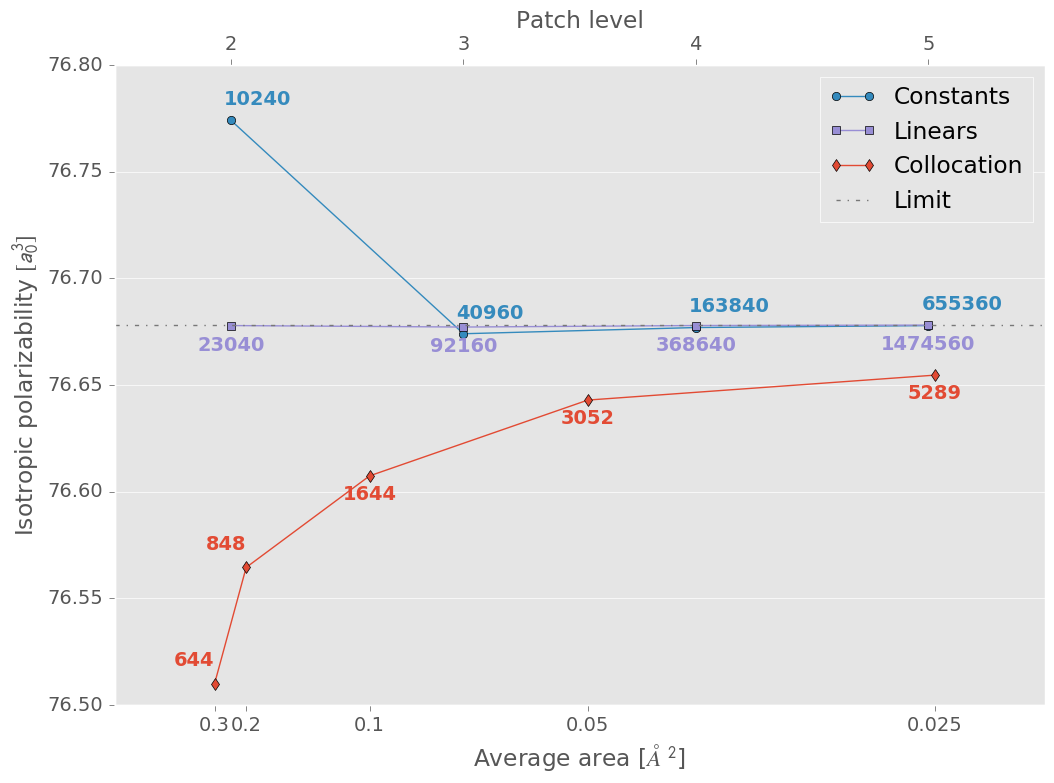
\includegraphics[width=\textwidth]{gfx/wemlin/alpha_convergence.png}
  \caption[Convergence of $\alpha_\mathrm{iso}$ with respect to the number of molecular
  electrostatic potential (MEP) evaluation points on the cavity surface.]
  {Convergence of $\alpha_\mathrm{iso}$ with respect to the number of
   molecular electrostatic potential (MEP) evaluation points on the cavity
   surface.
   The values reported are in $a_0^3$ and refer to benzene.
   The lower axis reports the average area for the collocation
   tesselation, while the upper axis refers to the patch level in the
   wavelet Galerkin discretization. The annotation report the number of
   MEP evaluation points.
   The compression parameter triplet was set to $a = 2.5,\ d^\prime =
   2.0,\ b = 0.01$ for the piecewise constant wavelets and to $a = 2.5,\
   d^\prime = 3.0,\ b = 0.01$ for piecewise bilinear wavelets.
   The limit value is extrapolated from the results obtained from the
   piecewise bilinear wavelet Galerkin scheme.}
  \label{fig:alpha_convergence}
\end{figure}

Finally, the interface to \LSDALTON was later released in the 2016 version,
providing \acs{PCM} capabilities to the software package.

\refstepcounter{dummy}
\addcontentsline{toc}{section}{Non homogeneous environments}
\section*{Paper III: Non homogeneous environments}

Continuum solvation models offer a simple route to the treatment of non
homogeneous environments.
The general integral equation formulation exposed in Chapter~\ref{ch:CSM} is in
fact transparent with respect to the definition of the Green's function for the
space portion exterior to the cavity.
As already shown by \citeauthor{Cances1998-og}, the same mathematical formalism can easily accommodate
environments characterized by distance-dependent or anisotropic Green's functions, such as those for
ionic liquids (in the weakly interacting regime described by the linearized Poisson--Boltzmann equation)
and liquid crystals, respectively.
\citeauthor{Frediani2004-er} showed that a numerical representation of the
Green's function is sufficient to obtain the boundary integral operators in the
\acs{PCM} integral equation.
The authors introduced a numerical integration procedure to calculate the
Green's function for an environment characterized by spatially varying, yet
cilindrically symmetric, permittivity functions: a model for planar diffuse interfaces.

In this work, a similar procedure was introduced to tackle diffuse interfaces
in spherical symmetry.
In contrast to previously existing work, our implementation offer a more robust
treatment of thin interfaces, with a rather generic functional form for the
permittivity profile.
We thoroughly analyzed the necessity for the \emph{a posteriori} removal of the
Coulomb singularity from the computed Green's function and its efficient
implementation.
Interface width and curvature influence the transfer of ions and molecules across
spherically symmetric interfaces and peculiar properties may arise.
In this work, we analyzed both effect on the water-vapor and oil-water transfer
of \ce{Li+}, \ce{Br-}, acetone, \emph{para}-nitroaniline and the L0 dye.
Nonelectrostatic interactions were not included in our implementation, although
they have been proved to be crucial for non homogeneous
environments.~\autocite{Mozgawa2014-ad}
Nevertheless our implementation represents a first significant step in the continuum treatment
of such nontrivial environments.

\begin{figure}[tb]
  \centering
  \begin{subfigure}[t]{.49\linewidth}
  \centering
  % Figure8a <--> dipole_acetone_perpendicular
  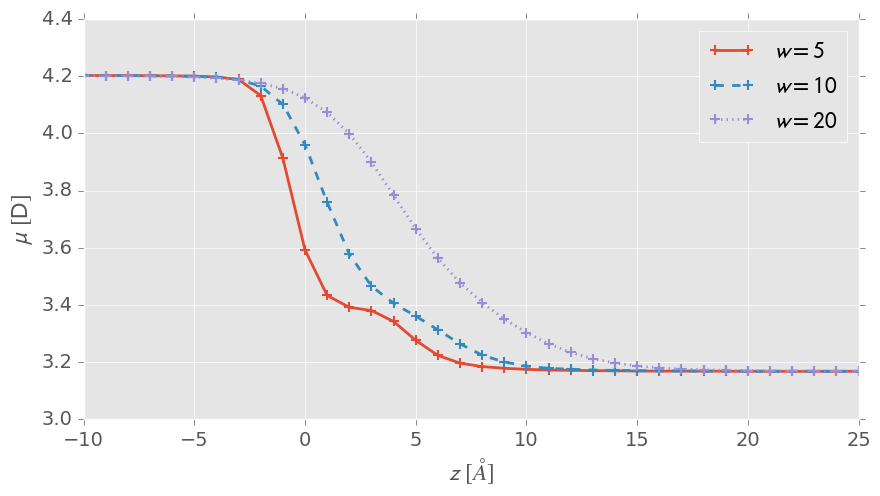
\includegraphics[width=\textwidth]{gfx/spherical/width.png}
  \caption{Width effect}
  \label{fig:profile_dipole_acetone_width}
  \end{subfigure}
  ~
  \begin{subfigure}[t]{.49\linewidth}
  \centering
  % Figure8b <--> curv_fullprofile_dip_acetone
  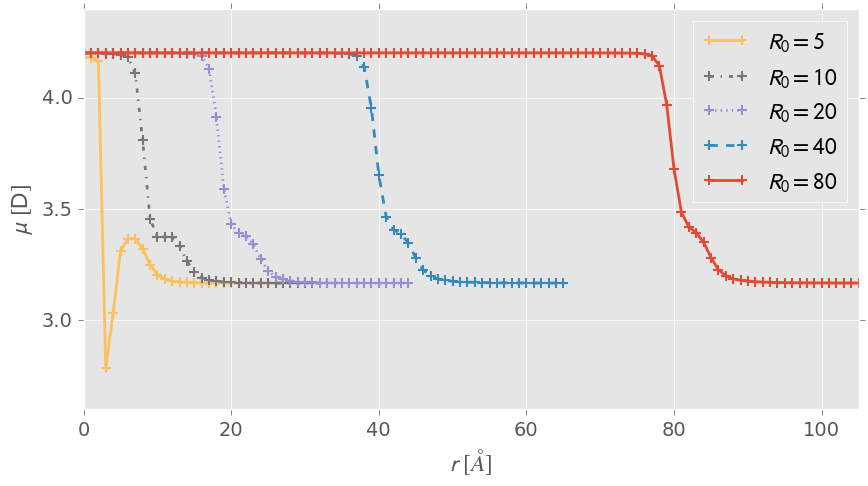
\includegraphics[width=\textwidth]{gfx/spherical/radius.png}
  \caption{Radius effect}
  \label{fig:profile_dipole_acetone_fullprofile}
  \end{subfigure}

  \begin{subfigure}[t]{.49\linewidth}
  \centering
  % Figure8c <--> curv_dip_acetone
  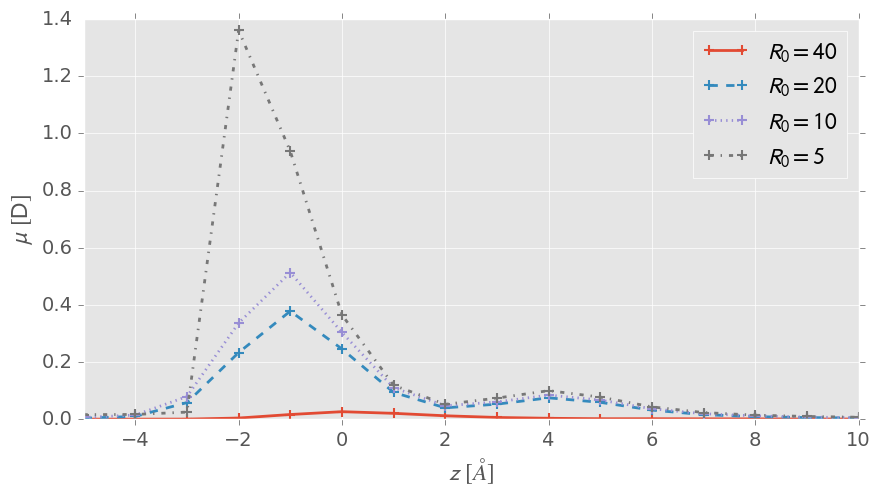
\includegraphics[width=\textwidth]{gfx/spherical/curvature.png}
  \caption{Curvature effect}
  \label{fig:profile_dipole_acetone_curvature}
  \end{subfigure}
  \caption[Width, radius and curvature effect on the dipole moment of acetone for water-air droplet phase transfer.]
  {Dipole moment profiles for acetone (with dipole moment
  perpendicular to the interface) transfer at water droplet in air, for
  varying interface widths, values of $R_0$ and the curvature effect on
  dipole moment, respectively.}
  \label{fig:profile_dipole_acetone}
\end{figure}

I contributed most of the theoretical work for this paper, based on early drafts from coauthors
Ville Weijo and Hui Cao. In particular, I derived the separation of
the Coulomb singularity in its final form.
Moreover, I contributed the implementation and testing of the Green's function code.
The interface to the \LSDALTON program package, developed within paper II, was
also used for this paper.
I wrote the first draft of the paper and coordinated all subsequent editing stages.

\refstepcounter{dummy}
\addcontentsline{toc}{section}{Relativistic calculation of EPR and pNMR parameters in solution}
\section*{Paper IV: Relativistic calculation of EPR and pNMR parameters in solution}

\refstepcounter{dummy}
\addcontentsline{toc}{section}{Open-ended self-consistent field response theory in solution}
\section*{Paper V: Open-ended self-consistent field response theory in solution}
